\documentclass[output=paper]{langscibook}
\ChapterDOI{10.5281/zenodo.6811462}
\author{Alison Porter\affiliation{University of Southampton\orcid{}} and Suzanne Graham\affiliation{University of Reading}\orcid{}}
\title[Research in primary languages]{Research in primary languages: Contribution to teacher professional development}
\abstract{The teaching of a second/foreign language in primary school has become a global phenomenon. Nevertheless, the scant evidence that exists about primary school teachers’ knowledge and beliefs about language pedagogy suggests that these are often influenced by their own experiences and ``lay wisdom'' rather than by re\-search-in\-formed principles. Furthermore, bringing about shifts in the knowledge and beliefs of busy in-service teachers is a challenge. This chapter begins by outlining what is already known about primary language teachers’ beliefs, and what key research-informed principles might be important for them to know and understand. It then considers the creation and impact of an online training initiative designed to develop teachers’ understanding of primary languages pedagogy and practice. Drawing on both quantitative and qualitative data from teacher participants in a Massive Online Open Course (MOOC), we discuss whether the initiative resulted in changes in teachers’ understanding and beliefs, and to what extent the methods used in the online materials facilitated any development. The chapter concludes by considering the implications of the study for models of primary school language teacher development and areas for future research.}


\begin{document}
\maketitle 

\section{Teacher beliefs about early language learning}\label{sec:porter:1}

Early instructed language learning is a field where, perhaps more than any other in the broader domain of language education, there exists a number of commonly held lay beliefs that misalign with what research proves or disproves.\footnote{We have adapted \citegen{Laurillard2012} framework labels from ``teacher'' to ``instructor'' to distinguish between MOOC educators (instructors) and our participants who were teachers/teacher educators.}  If teachers themselves hold such beliefs, this may impact on their ability to provide young learners with appropriate instruction. Furthermore, teachers of young language learners (ToYLLs) are arguably often quite different from other kinds of teachers, and also from language teachers working in secondary schools. Most did not start their teaching career in the area of languages, but have moved into it, often without much specialist training (\citealt{GartonEtAl2011}). Alternatively, they may have trained as a generalist primary school teacher, with only a small portion of their pre-service period devoted to languages. Any lack of pedagogical knowledge on their part would not therefore be altogether surprising.

Research into the beliefs and pedagogical knowledge and practices of teachers of young language learners can be summarised as follows:

First, a common belief is that the younger learners are when they start to receive language instruction at school, the more proficient they will become. Relatedly, it is commonly thought that they all make rapid progress, absorbing language ``like a sponge'', effortlessly and with enthusiasm, to borrow a commonly used expression. A large majority (92\%) of the respondents in \citegen{Barrios2014} questionnaire study of pre-service language teacher beliefs viewed young learners as more able to learn a language than adults. This was echoed by a study of in-service and pre-service teachers in Turkey by \citet{KocamanCansiz2012}.

\begin{sloppypar}
Second, research suggests misunderstanding and misconceptions among researchers and ToYLLs regarding implicit vs explicit learning, and the balance needed between speaking and listening on the one hand and literacy-based learning and grammatical knowledge development on the other. Several studies note teacher misconceptions around what is meant by Communicative Language Teaching (\citealt{Butler2005,GartonEtAl2011}). Others highlight a lack of knowledge of developmental theory (\citealt{Hild2017,Rea-DickinsGardner2000}) and of pupils’ increasing ability to deal with abstract concepts as they grow older. For example, in a study of in-service teachers in Spain, \citet{Roothoft2017} found that ToYLLs paid little attention to reading and writing or grammar in their instruction. The author argues that teachers’ own negative experiences as learners, where they experienced a heavy emphasis on grammar, led them to want to teach in the opposite way. Likewise, pre-service and in-service teachers in \citet{KocamanCansiz2012} attached different degrees of importance to teaching English spelling and grammar (36\% of the former thought such instruction was unnecessary, against 63\% of the latter), indicating overall levels of uncertainty as to what might be most appropriate. Around a third of \citegen{Barrios2014} participants also felt, however, that it was important to correct learners’ errors in order to eradicate them quickly, before they became entrenched, suggesting weak knowledge of language development issues. \citet{Liao2007} reported similar views among 99 teachers in Taiwan (21 pre-service, 78 in-service). Overall, it seems then that many ToYLLs lack a clear understanding of research-supported principles for teaching young learners.
\end{sloppypar}

\subsection{What might we hope primary MFL teachers would know?}\label{sec:porter:1.1}

While it would probably be unreasonable to expect from ToYLLs in-depth and extensive knowledge of early language learning research, given evidence of teachers’ difficulty in accessing research publications (\citealt{MarsdenKasprowicz2017}), it is possible to identify some key evidence-based principles useful for them to know. These might be grouped into the broad, overlapping themes of (i) learner progression (ii) motivation and (iii) literacy and grammar development.

First, in contrast to the view that early language learning is quick and easy, in reality we know that an earlier start does not of itself lead to greater proficiency. For example, studies indicate that learners who start later can catch up and achieve higher proficiency levels, especially in grammar (\citealt{MylesMitchell2012}). Early language learning needs the right conditions to be successful, particularly in respect of the amount and quality of second language input learners receive in the classroom (\citealt{GrahamEtAl2017,MitchellMyles2019}). Rather than being an effortless process, early language learning requires learners to experience language in different modalities, and to have meaningful and repeated encounters with language (\citealt{MitchellMyles2019,MylesMitchell2012,Porter2020}). Likewise, learners can progress at different rates, with some experiencing more difficulties than others (\citealt{CableEtAl2010,GrahamEtAl2017,Porter2020}).  Importantly, far from being a fast process, progress in early language learning, while statistically significant, is very slow; primary school learners made small gains in oral and written proficiency (\citealt{Courtney2014,GrahamEtAl2017,MitchellMyles2019,MylesMitchell2012,Porter2020}), especially in terms of creative sentence building and moving away from the use of memorised expressions (\citealt{CableEtAl2010}).

Second, language learning motivation, by and large, tends to be high among younger learners (\citealt{CableEtAl2010}). Yet not all young learners are highly motivated. For example, \citet{CourtneyEtAl2017} found that around 20\% of primary school learners in their study had low levels of motivation and were fairly pessimistic about their ability to make progress in the future.  Teaching that does not provide learners with that sense of progression is unlikely to foster high levels of motivation. The desire to communicate is an important motivator for young learners, meaning that instruction that enables them to do that from an early stage, by, for example, teaching language in chunks, is more likely to nurture their sense of achievement (\citealt{CableEtAl2010}). As they progress, learners then become able to break these chunks down and use them more creatively and independently (\citealt{MylesEtAl1998}). Furthermore, motivation among young learners is far from static -- as is the case with other age groups, it fluctuates over time and tends to change in nature with age. Given the importance of motivation for language learning outcomes (\citealt{DörnyeiSkehan2003}), teachers need to understand its development.

Third, while it is likely that language learning at an early age draws heavily on implicit learning mechanisms (\citealt{DeKeyser2003}), the limited amount of classroom time usually available in primary school (\citealt{GrahamEtAl2017}) means that some attention to explicit knowledge development is needed as well. Indeed, as learners approach early adolescence and become more capable of abstract thought and reflection, some explicit grammar instruction can speed up their progress, especially if they have higher levels of language analytic ability (\citealt{KasprowiczEtAl2019,Roehr-BrackinTellier2019}). Furthermore,  in Communicative Language Teaching (CLT) oral and aural skills are foregrounded, but excluding literacy entirely represents a misunderstanding of CLT and learners’ developmental needs. Indeed, attention to phonics instruction and writing development can go hand in hand with teaching that is focused on oral development, especially when integrated with interesting and motivating texts and tasks (\citealt{Porter2020}).

\subsection{ToYLL's development}\label{sec:porter:1.2}

Given that ToYLLs may have received relatively little training either pre-service or in-service, and that there seems to be a mismatch between teacher beliefs and research findings regarding early language learning, there is thus a need in many contexts to try to bridge that gap through research-informed continuous professional development (CPD). A fairly large body of research on language teacher cognition suggests that evidence-based CPD can have mixed levels of impact on language teachers (for a recent summary, see \citealt{MacaroEtAl2015}). That, however, seems to depend not only on the type of CPD offered, but also on how ``impact'' is defined and assessed. Does it imply complete change or modification (\citealt{CabarogluRoberts2000}) of both beliefs and classroom practice, or just one of those? We share the view of \citet[129]{MacaroEtAl2015} that research-based CPD is important because ``developing teachers’ theoretical and research-based knowledge improves [their] ability to make principled pedagogical decisions, as well as their insights into the complexity of the learning process''.

Furthermore, a number of reviews draw together common characteristics of effective forms of research-based CPD and adult learning programmes. Synthesising several studies to determine the characteristics of effective teacher CPD, \citet[240]{Cordingley2015} highlights the use of
(1) evidence and research expertise, especially to inform teacher planning,
(2) peer support,
(3) collaboration and dialogue, and
(4) ``enquiry-oriented learning''. Community support is also at the heart of Laurillard’s work on conversational frameworks for adult learning, especially of the kind based on the use of learning technologies. That framework outlines four cycles of what Laurillard calls a ``learning conversation'': instructor communication, instructor practice/modelling, peer communication and peer modelling (\citealt{Laurillard2012}). Cycles occur iteratively, and in each cycle learning is portrayed as a process which
a) involves instructor and learner interaction and
b) develops conceptual knowledge and practical action (\citealt[87]{Laurillard2012}). The instructor communication cycle is grounded in social constructivism, the view that ``individuals are active participants in the creation of their own knowledge'', particularly through interaction with others (\citealt[67]{DavisEtAl2017}), and concerns learning at the conceptual level. Instructor practice and modelling cycles reflect experiential learning and involve opportunities to engage in practical action or to experience instructor modelling, both of which will support learning. Finally, the peer communication and modelling cycles recognise the Vygotskyan social constructivist view of learning and acknowledge a role for interaction and exchange of ideas, experiences, and also modelling practice (\citealt{Laurillard2012}).

Different types of media and teaching technologies can support these cycles (\citealt{Laurillard2002}). Narrative media forms, such as video or print, are suited to instructor communication of concepts. Interaction can include ``discussing'', ``debating'', ``experimenting'' and ``practising'' whereby the learner interacts with the instructor and other learners, using, for example, online collaboration tools such as wikis. In the practice cycle, the learner tries out ideas and modifies them in light of feedback (from the instructor and/or peers) and experience, perhaps via a simulation or real-life environment (\citealt{Laurillard2002}). The framework is designed to offer a way of checking that any learning environment, particularly digital ones, offers the optimal conditions for learners to generate ``articulations and actions'' and to ``modulate their concepts and actions'' (\cites[]{Laurillard2007}[94]{Laurillard2012}). In teacher education, for example, this might involve creating a resource based on instructor input, receiving initial feedback on it from peers, then trying out a modified version in the classroom. It also forms the basis of a widely-used platform for adult learning, including learning by teachers: FutureLearn’s MOOC\footnote{\url{https://www.futurelearn.com}}. FutureLearn MOOCs typically include a number of ``steps'' that the learner works through and marks as ``complete''.

\begin{sloppypar}
The study in this chapter describes a three-week, research-informed CPD MOOC which commenced in  July 2020  during the COVID-19 pandemic. MOOCs are free and impose no limit on the number of participants.
\end{sloppypar}

The extent to which CPD based on the above principles can influence the beliefs and practices of teachers of early language learning is the focus of the study we describe below, addressing the following research questions: 

\begin{enumerate}
  \item To what extent did research-informed CPD input bring about changes in beliefs/knowledge and changes (planned or enacted) in teaching practice?
  \item Which MOOC step types, based on Laurillard’s communication/modelling cycles for learning environment design, promoted the most learner engagement?
\end{enumerate}

\section{The study}\label{sec:porter:2}
\subsection{MOOC design: Guiding principles}\label{sec:porter:2.1}

Evidence of scant opportunities for primary school teachers to engage with high-quality languages CPD (\citealt{TinsleyBoard2017}) led the research team (Alison Porter, Florence Myles and Suzanne Graham) to develop a Massive Online Open Course (MOOC) called ``Teaching Languages in Primary Schools: Putting Research into Practice''. The course was hosted by the British digital education platform, FutureLearn.

MOOC research had identified that short courses with a maximum of 5 study hours per week were optimal for CPD purposes (\citealt{Laurillard2014}), so this course aimed to offer participant teachers/teacher educators structured tasks with accessible readings scheduled over three weeks.

The overarching premise of the course was to~support primary school practitioners to develop their pedagogic knowledge through the exploration of early foreign language learning research findings. Teachers were then encouraged to use this knowledge to make principled pedagogic decisions for example through making suggestions for pedagogic scenarios (``what would you do?''). The MOOC aimed to target both pre-service and in-service teachers as well as teacher educators. Bearing in mind this potentially heterogenous cohort, it was agreed that weekly key research ``messages'' were presented which were related to gaps in teacher beliefs derived from the TOYLLs research literature (\sectref{sec:porter:1}). The messages were then aligned with clearly defined pedagogic principles (\tabref{tab:porter:1}).


\begin{table}
\begin{tabularx}{\textwidth}{lQ}
\lsptoprule
\multicolumn{2}{p{\linewidth-4\tabcolsep}}{{\itshape Week 1 message:} Younger learners are not necessarily better at language learning}\\
Principle 1 & Young children will benefit from different kinds of teaching and learning activities as they progress through primary education.\\
Principle 2 & Pedagogy for young learners should transition from an emphasis on fun and repetition to more structured, reflective opportunities for learning.\\
Principle 3 & A sense of progression and achievement becomes increasingly important in upper primary classrooms.\\
\midrule
\multicolumn{2}{p{\linewidth-4\tabcolsep}}{{\itshape Week 2 message:} Getting beginner learners to use language for communication is beneficial}\\
Principle 4 & Teaching fixed expressions can lay the foundation for later creative use.\\
Principle 5 & Vocabulary and chunk learning needs multimodal learning experiences with regular practice.\\
Principle 6 & Explicit awareness-raising of language patterns could help progression in grammar.\\
\midrule
\multicolumn{2}{p{\linewidth-4\tabcolsep}}{{\itshape Week 3 message:} Teaching FL literacy can encourage independent and creative language use}\\
Principle 7 & FL literacy instruction should be systematic and integrated.\\
Principle 8 & Teach learners to recognise words through phonics instruction and learning whole words.\\
Principle 9 & Rich and meaningful encounters with text are important for FL literacy progress, FL motivation and engagement.\\
\lspbottomrule
\end{tabularx}
\caption{Weekly research messages and pedagogic principles}
\label{tab:porter:1}
\end{table}

Weekly activities were mapped against three cycles adapted from Laurillard’s Conversational Framework 2012 as outlined in \sectref{sec:porter:1.2}. We used her Instructor Communication and Instructor Practice/Modelling terms, and combined her Peer Communication and Peer Modelling into one cycle category. As illustrated in \sectref{sec:porter:2.1.3}, we felt this combined third cycle reflected more accurately how, in our experience, teachers tend to discuss, share and demonstrate their ideas for practice in conversations where it is hard to separate communication and modelling. We were also aware that the steps deemed to represent peer activities included video ``teacher stories'' in which non-participant teachers illustrated examples of their own teaching practices and resources. Participant comments were then elicited at the end of each story -- this meant that modelling and communication were intrinsic, we felt, to these steps. We hoped thereby to reflect Laurillard’s view of learning as an iterative process through which learner concepts (knowledge) and practice (application of knowledge) are developed, while also adapting her model to suit our particular learners. By equipping learners with the knowledge to make principled pedagogic decisions, the MOOC aimed to motivate learners, stimulate discussion, experimentation, enactment and adaptation of concepts and practices. 

\subsubsection{Cycle one: Instructor communication}\label{sec:porter:2.1.1}

In cycle one, the instructor and learner engaged in dialogic behaviour to support learner acquisition of new child development, linguistic and/or pedagogic concepts or research findings. The instructor introduced and explained new concepts whilst the learner was encouraged to articulate understanding and ask questions relating to the concept and/or their practice (\citealt{Laurillard2012}). For example, in week 1 learners explored the research finding that context is key in determining the effects of age in linguistic outcomes, and the concept that primary school language learning takes place during a time of huge cognitive, social and emotional change. \tabref{tab:porter:2} identifies which particular steps in the MOOC formed part of the instructor communication cycle. Note that \citeauthor{Laurillard2012}’s framework allows for an ``extrinsic feedback'' (\citeyear[95]{Laurillard2012}) phase in the instructor communication cycle which, in the MOOC, was provided through facilitator responses to weekly comments.

\begin{table}
\begin{subtable}{\textwidth}
\caption{Week 1}
\label{tab:porter:2a}
\begin{tabularx}{\textwidth}{QQ}
\lsptoprule
{Step title} & {Step content}\\
\midrule
Young learners' motivation and engagement in language learning* & Research findings video -- knowledge and explanation\\
\tablevspace
 Language learning at a time of developmental change* &  Research findings reading~\citep{TellierGraham2018} with comprehension questions -- knowledge and understanding\\
\tablevspace
 Revisiting the principles* &  Reminder of pedagogic principles in research video\\
 \tablevspace
 Test your learning &  Check knowledge -- memory and understanding\\
 \tablevspace
 Reflection on week’s content* &  Review key learning points -- knowledge and understanding\\
\lspbottomrule
\end{tabularx}
\end{subtable}\bigskip\\
\begin{subtable}{\textwidth}
\caption{Week 2}
\label{tab:porter:2b}
\begin{tabularx}{\textwidth}{QQ}
\lsptoprule
{Step title} & {Step content}\\
\midrule
 The potential for achievement in primary languages classrooms* &  Research findings reading with comprehension questions -- knowledge and understanding\\
 \tablevspace
 Revisiting this week's pedagogic principles* &  Reminder of pedagogic principles in research video\\
 \tablevspace
 Test your learning & Check knowledge -- memory and understanding\\
 \tablevspace
 Reflection on week’s content* &  Review key learning points -- knowledge and understanding\\
\lspbottomrule
\end{tabularx}
\end{subtable}
\caption{\label{tab:porter:2}Instructor communication cycle week 2: Total steps = 14}
\end{table}

\begin{table}
\ContinuedFloat
\begin{subtable}{\textwidth}
\caption{Week 3}
\label{tab:porter:2c}
\begin{tabularx}{\textwidth}{QQ}
\lsptoprule
{Step title} & {Step content}\\
\midrule
 The role of foreign language literacy in supporting language learning* &  Research findings video -- knowledge and explanation\\
 \tablevspace
 Developing literacy in a foreign language* &  Research findings reading with comprehension questions -- knowledge and understanding\\
 \tablevspace
 Revisiting this week’s pedagogic principles* &  Reminder of pedagogic principles in research video\\
 \tablevspace
 Test your learning & Check knowledge -- memory and understanding\\
\lspbottomrule
\end{tabularx}
\end{subtable}
\caption{Instructor communication cycle week 2: Total steps = 14}
\end{table}

\subsubsection{Cycle two: Instructor practice and modelling}\label{sec:porter:2.1.2}

Cycle two explored how the instructor ``influences the learners’ internal cycle at the practice level'' by providing opportunities to encourage practical action linked to underpinning concepts \citep[89]{Laurillard2012}. This cycle included instructor modelling to guide adaptation of actions and was categorised as an instructor-led cycle because the participants were not required to act upon concepts or findings i.e. whilst they reflected upon the information in the cycle, they did not yet have to offer any examples of relevant pedagogic tools or practical actions.

In the MOOC, this cycle did include activities which gave participants opportunities to experiment with practical solutions. This involved hypothetical scenarios where participants were asked to offer pedagogic suggestions to a fictional colleague, opportunities to reflect on current practice in light of recently explored concepts, and, finally, tasks to evaluate other teachers’ practices by linking these to theoretical evidence and principles (\tabref{tab:porter:3}).


\begin{table}
\begin{tabularx}{\textwidth}{p{.1\textwidth}lQ}
\lsptoprule
{Week} & {Step title} & {Step content}\\
\midrule
\multirow[t]{3}{=}{1, 2 \& 3} & What would you do? & Modelling: Hypothetical scenario created to elicit principled participant suggestions for practice. \\
\tablevspace
 & What do you do?* & Practice: Linking existing practice to underpinning concepts\\
 \tablevspace
 & Evaluator Task & Modelling: Develop understanding by~examining practice and linking to evidence and principles\\
\lspbottomrule
\end{tabularx}
\caption{Instructor practice/modelling cycle: Total steps = 9}
\label{tab:porter:3}
\end{table}

\subsubsection{Cycle three: Peer communication and modelling}\label{sec:porter:2.1.3}

In this cycle, learners collaborated to offer comments, alternative suggestions and critiques. Modelling, in this phase, involved use of peer modelling to modulate a learner’s practice. \tabref{tab:porter:4} shows how MOOC participants shared experiences and reflections on key concepts and practical solutions. Participants were also encouraged to listen to teacher stories (videos) in which practising primary FL teachers explained how they had adapted their pedagogies in line with theoretical and empirical evidence. Participants were invited to reflect on this model of research-informed adaptations to practice.

\vfill
\begin{table}[H]
\caption{Peer communication and modelling cycle: Total steps = 19}
\label{tab:porter:4}
\begin{subtable}{\textwidth}
\caption{Week 1}
\label{tab:porter:4a}
\begin{tabularx}{\textwidth}{QQ}
\lsptoprule
{Step title} & {Step content}\\
\midrule
 Children love learning languages and they're so good at it! Do you agree? &  Communication: Elicit~teachers’ existing beliefs and understandings~\\
 \tablevspace
 Do you teach culture and language? & Communication: reflection on concepts and practice\\
 \tablevspace
 Karen’s story: Making French fun &  Modelling: Teacher-led account of practice linked to pedagogic principles~\\
\tablevspace
 Claire’s story: Engaging emotions in German* &  Modelling: Teacher-led account of practice linked to pedagogic principles~\\
 \tablevspace
 Reflector Task & Communication: Link knowledge and practice:~Examining~teachers’~practices~against principles~\\
 \tablevspace
 Innovator Task & Modelling: Design an activity in line with principles. Feedback from participants and facilitators. \\
\lspbottomrule
\end{tabularx}
\end{subtable}
\end{table}
\vfill\pagebreak

\begin{table}
\ContinuedFloat
\caption{Peer communication and modelling cycle: Total steps = 19}
\begin{subtable}{\textwidth}
\caption{Week 2}
\label{tab:porter:4b}
\begin{tabularx}{\textwidth}{QQ}
\lsptoprule
{Step title} & {Step content}\\
\midrule
How can we encourage language use in beginner young learner classrooms? &  Communication: Elicit~teachers’ existing beliefs and understanding~\\
\tablevspace
 What language outcomes are expected in your setting? &  Communication: reflection on concepts and practice\\
 \tablevspace
 Sarah's story 1 -- The learning journey: knowing your destination &  Modelling: Teacher-led account of practice linked to pedagogic principles~\\
 \tablevspace
 Sarah's story 2 -- The learning journey:~stepping stones~to language use &  Modelling: Teacher-led account of practice linked to pedagogic principles~\\
 \tablevspace
 Clare's story -- The learning journey: making and measuring progress &  Modelling: Teacher-led account of practice linked to pedagogic principles~\\
 \tablevspace
 Reflector Task & Communication: Link knowledge and practice. Examine teachers’ practices against principles~\\
 \tablevspace
 Innovator Task & Modelling: Design an activity in line with principles. Feedback from participants and facilitators. \\
\lspbottomrule
\end{tabularx}
\end{subtable}
\end{table}

\begin{table}
\ContinuedFloat
\caption{Peer communication and modelling cycle: Total steps = 19}
\begin{subtable}{\textwidth}
\caption{Week 3}
\label{tab:porter:4c}
\begin{tabularx}{\textwidth}{QQ}
\lsptoprule
{Step title} & {Step content}\\
\midrule
 How can we foster independence and autonomy in young learner classrooms? & Communication: Elicit~teachers’ existing beliefs and understandings~\\
 \tablevspace
 How can you use FL literacy with beginner learners? & Communication: reflection on concepts and practice\\
 \tablevspace
 Becca's story: Phonics in a foreign language & Modelling: Teacher-led account of practice linked to pedagogic principles~\\
 \tablevspace
 Claire and Susi: Using stories to teach language & Modelling: Teacher-led account of practice linked to pedagogic principles~\\
 \tablevspace
 Reflector Task & Communication: Link knowledge and practice; Examine teachers’ practices against principles~\\
 \tablevspace
 Innovator Task & Modelling: Design an activity in line with principles. Feedback from participants and facilitators. \\
\lspbottomrule
\end{tabularx}
\end{subtable}
\end{table}

\subsection{Participants}\label{sec:porter:2.2}

MOOCs are often delivered in ``runs'', that is a period of time when the course is open to learners. This can happen several times a year, and the data for this study came from the first MOOC run in July 2020. 4931 participants joined the course, of those, 3435 (69.7\%) became ``learners'', meaning that they \textit{viewed} at least one step in the MOOC and 2338 became ``active learners'', meaning that they \textit{marked as complete} at least one step. Learners came from 140 countries (\figref{fig:porter:1}).

\begin{figure}
\includegraphics[width=\textwidth]{figures/a8PorterGraham-img001.png}
\caption{Map showing participant location for MOOC (NB: shading indicates global joiner rates, FutureLearn does not provide a key). The map is reproduced with permission, © FutureLearn 2022, all rights reserved.}
\label{fig:porter:1}
\end{figure}

MOOCs are widely known to experience a degree of learner attrition -- completion rates for courses are generally below 13\% (\citealt{OnahEtAl2014}) and this course was no exception. However, whilst the MOOC noted a steady decline in visits, completed steps and comments over the course of three weeks (\tabref{tab:porter:5}), its completion rate of 18.8\% (or 649 participants who completed more than 90\% of steps) was slightly higher than the norm.


\begin{table}
\begin{tabular}{l *3{r}}
\lsptoprule
& {Week 1} & {Week 2} & {Week 3}\\
\midrule
Learners’ visiting steps & 3429 & 1134 & 931\\
Active learners & 2318 & 1030 & 824\\
Visited steps & 29769 & 15803 & 13189\\
Completed steps & 24553 & 14319 & 11872\\
Average completed steps per user & 10.59 & 13.9 & 14.41\\
Comments & 7397 & 3683 & 2817\\
\lspbottomrule
\end{tabular}
\caption{Learner activity summary\label{tab:porter:5}}
\end{table}

In week 1 over 82\% of visited steps were completed (that is, marked as complete by the participant). In weeks 2 and 3 step completion rates rose to 90\%, possibly linked to the high rate of attrition of active learners between week 1 and 2 (33\% and 44\% respectively).\largerpage

Throughout the course, a range of on-platform and off-platform data were collected as outlined below, primarily to explore change in teacher understanding, knowledge and practices and hence answer our two research questions.

\subsection{Data coding and analysis: Qualitative data}\label{sec:porter:2.3}
\subsubsection{Participant platform comments}\label{sec:porter:2.3.1}

As learners progressed through MOOC steps, they were invited to post comments on the platform, respond to questions and discuss ideas or experiences. They were supported by two online facilitators (both experienced language teachers and teacher educators) who engaged with participant questions, ``liked'' or pinned useful and/or pertinent learner posts and encouraged interaction. Teachers are known to be particularly active in online MOOC discussions and forums and contribute in a ``genuinely interactive'' manner (\citealt[6]{Laurillard2014}). During this MOOC, 3445 ``active learner'' participants (see \sectref{sec:porter:2.2}) posted a total of 13897 comments online. FutureLearn’s privacy policy means that these comments, which are each linked to a unique participant identifier, cannot be quoted directly, but they can be analysed for trends and broad content. The researchers anticipated that each step would yield rich data which could be used to explore the learning process including how participants engaged with new knowledge in the form of research findings and practical reflection and/or experimentation.

A coding framework was developed to capture different levels of change such as teacher espoused beliefs expressed in verbal or written formats and planned or enacted changes in practice derived from enacted beliefs (\citealt{FivesBuehl2012}) (Appendix~\ref{app:porter:b}). Despite our original intention to encourage and facilitate practical experimentation, many teachers were working under lockdown conditions and teaching online, and participants, especially in the UK, were often not actively teaching languages. We therefore decided to make a distinction between planned practical change and change that had actually been implemented. Analysis was intended to be both inductive and deductive. In other words, coders worked to a ``theory-driven, deductive approach'', applying codes from existing theoretical frameworks but also had the flexibility to respond inductively to novel concepts expressed in the data. Following this, coded transcripts were then investigated for themes showing emerging patterns in the coded data (\citealt[2]{XuZammit2020}).

From the total of 49 steps, a smaller sub-sample of 12 were initially coded. These steps (marked with an asterisk in Tables~\ref{tab:porter:2}--\ref{tab:porter:4}) were deemed likely, due to learning design elements, to elicit instances of changes in beliefs, knowledge and/or practice, and help answer our first research question. A team of analysts applied the codes \citep{TellierGraham2018} to the sub-sample of 12 steps in an initial wave of coding, covering 3011 comments from a total of 13897 (21.7\%). The appendix also includes examples of how ``change'' was identified in the coding. Any one comment could be coded under multiple codes, for example a comment ``I’m going to embrace teaching reading strategies now that I’ve found out about the research exploring benefits of French literacy instruction'' would have been coded as
(1) planned changes in teaching practice to support FL reading and
(2) explicit reflections on MOOC research content/articulation of research findings. Samples of coding in 4 steps (33\% of the total steps) were revisited 8 weeks after the first coding round. This process was conducted by the first author who had devised and trialled the coding framework with the coding team. This process resulted in a small number of changes in coding ($n = 12$).

\subsubsection{Participant off-platform comments}\label{sec:porter:2.3.2}

At the end of each MOOC week, participants were asked to opt-in to an online questionnaire which aimed to explore in more detail the development of their understanding, knowledge and practices. The questionnaire involved statements relating specifically to that week’s contents, and participants were asked to rate their agreement with these statements using a 5-point Likert scale (1 = strongly agree, 5 = strongly disagree). For example: ``I have learnt something new about how children’s learning changes between ages 7 and 11''.  They were also given space to add more information about their perceptions of changes in beliefs or practice if they wished.

A total of 476 questionnaires were completed during the July MOOC course (238 in week 1; 126 in week 2 and 112 in week 3), with 2,426 comments to open-answer questions. The latter form the focus of our exploration of developing understanding and changes in practice in \sectref{sec:porter:2}.

The majority of respondents to this round of data collection were teachers (approximately 90\%), of which there were a small minority of teacher trainers (approximately 19\%).

\subsection{Data coding and analysis: Quantitative data}\label{sec:porter:2.4}

These comments were analysed for insights into the level of engagement by the 3435 uniquely identified MOOC participants according to step type. Quantitative data included the following metrics, with step activity (step completion data) forming the main focus of our analysis.

\subsubsection{Step activity}\label{sec:porter:2.4.1}

It was envisaged that the step activity data could act as a proxy for learner behavioural engagement (\citealt{FredricksEtAl2004,GobertEtAl2015}) and/or perceived relevance of the step activity.

Files were downloaded from the platform which contained unique identifiers for each participant and the steps they had accessed. Date and time stamps were used to mark when a step was opened and then marked as complete, as evidence of behavioural engagement. An Excel file was created from these data, showing level of activity, for each participant and for each step. The following codes were used: 0~=~step opened not complete; 1~=~step opened and complete; 999~=~no entry for that unique identifier/step. The adapted Excel spreadsheets were then imported into SPSS for statistical analysis.

\subsubsection{Question response}\label{sec:porter:2.4.2}

This file contained data listed by participant unique identifier which itemised responses to multiple choice quizzes in the summary activities.

\subsubsection{Video viewing}\label{sec:porter:2.4.3}

This involved the collection of video download and view frequencies. These were not listed by participant but by step number.

\section{Results}\label{sec:porter:3}
\subsection{Research question 1}\label{sec:porter:3.1}

To what extent did research-informed CPD input bring about changes in beliefs/knowledge and changes (planned or enacted) in teaching practice?

\subsubsection{Changes in beliefs/knowledge}\label{sec:porter:3.1.1}
\begin{sloppypar}
The qualitative platform data showed that from the 12 steps analysed (see \sectref{sec:porter:2.4.1} steps marked with an asterisk) there were a total of 2982 counts of instances of change. Most of these counts related to modifications in teacher understanding, including new or adapted understandings, beliefs or knowledge, which amounted to 1755 (58.9\%) instances in total. In terms of changes in practice, there were fewer numerical counts of change. 610 instances (20.50\% of the comments analysed) demonstrated either planned or enacted changes in teaching practice.
\end{sloppypar}

A matrix coding query to find instances of intersections between change and step type was then run to determine any tendencies to reflect on MOOC related research by coded step. The frequency data showed that participants tended to discuss research findings with peers or facilitators most frequently (689 counts -- 23.10\% of comments); they then were more likely to articulate research findings (83 total counts; 12.0\% of the sub-group). There were 48 counts (6.97\% of sub-group comments) of participants requesting further clarification or explanation of research findings. 

Subsequent analyses using Nvivo frequency data showed that the instructor communication cycle steps were likely to generate the most recorded instances of changes in beliefs or understanding, as shown in \tabref{tab:porter:6}. However, it is important to note here that fewer steps were coded in the instructor practice/modelling and peer communication/modelling steps.


\begin{table}
\begin{tabularx}{\textwidth}{Qrrr}
\lsptoprule
{Change in teacher beliefs/understanding (total = 1755)} & {Week 1} & {Week 2} & {Week 3}\\
\midrule
Non-specific & 3 & 0 & 0\\
Nature of development in middle childhood & 180 & 4 & 0\\
Importance of progression for motivation & 134 & 12 & 3\\
Independent language use & 4 & 25 & 7\\
Learning of grammar & 1 & 169 & 4\\
Learning to read in the FL & 5 & 2 & 127\\
Learning to write in the FL & 1 & 0 & 5\\
Learning vocabulary & 6 & 79 & 15\\
Multimodality & 5 & 102 & 14\\
Phonics Understanding & 0 & 0 & 0\\
Planning for progression & 35 & 0 & 0\\
\midrule
Total instances of change & 374 & 393 & 175\\
\lspbottomrule
\end{tabularx}
\caption{Instances of change in beliefs/understandings reported in research findings video steps (instructor communication cycle)}
\label{tab:porter:6}
\end{table}

Areas with the highest counts – developmental change (10.48\%), progression for motivation (8.49\%), learning of grammar (9.91\%), multimodality (6.89\%), learning to read in the FL (7.64\%) represented the core themes in each week’s content. In other words, reported instances of developments in understanding and knowledge were closely linked to the key messages presented. Having said that, there were lower counts, in week 3’s video, for phonics understanding which formed a core part of the literacy content. This, it is suggested, could be due to participant demographic factors. 885 active learners reported the UK as their country of origin, and primary school teachers as well as wider education stakeholders in this country are likely to be conversant and confident with the concept of phonics instruction, which is widely practised in the early primary years. 

\subsubsection{Changes in planned or enacted practice}\label{sec:porter:3.1.2}

The research findings videos encouraged a relatively small number of instances where participants reported plans to adapt their practice (\tabref{tab:porter:7}).


\begin{table}
\begin{tabularx}{\textwidth}{Qrrr}
\lsptoprule
{Change in practice planned (total = 478)} & {Week 1} & {Week 2} & {Week 3}\\
\midrule
Unspecified & 4 & 2 & 1\\
To support grammar teaching & 0 & 16 & 0\\
To support independent language use & 1 & 7 & 3\\
To support language use & 4 & 5 & 2\\
To support motivation and/ or engagement & 66 & 0 & 0\\
To support reading & 1 & 0 & 47\\
To support use of multimodality & 1 & 6 & 1\\
To support writing & 0 & 0 & 3\\
\midrule
Total instances of planned practice & 77 & 36 & 57\\
\lspbottomrule
\end{tabularx}
\caption{Planned changes in practice by instructor communication cycle steps reported in research findings video steps}
\label{tab:porter:7}
\end{table}

 Unsurprisingly, comments tended to focus on the main theme in each week. The research videos were more likely to facilitate changes in knowledge and understanding than in practice, perhaps because participants needed more structured opportunities and guidance for the latter to happen. A matrix coding query across all steps showed that for planned practice (478 total comments) participants tended towards changes to support motivation (199 counts -- 41.63\% of total planned practice comments), reading (63 counts -- 13.18\% of total) and language use (53 counts -- 11.09\% of total).

\tabref{tab:porter:8} shows that far fewer cases of enacted practices were recorded but this was probably largely due to teachers working under lockdown conditions at the time of the course and, whilst in the UK teaching moved online, there tended to be much greater focus on ensuring core curriculum subjects such as mathematics, English and science were taught rather than languages. Frequency counts of enacted practice (54 total comments) demonstrated that participants implemented changes to support motivation (40.74\% of total enacted comments) and grammar teaching (7.41\% of total enacted comments). Most planned and enacted practice comments were generated by instructor communication steps (e.g. research videos, research readings and revisiting pedagogic principles).


\begin{table}
\begin{tabularx}{\textwidth}{Qrrr}
\lsptoprule
{Changes in practice enacted (total = 132)} & {Week 1} & {Week 2} & {Week 3}\\
\midrule
Unspecified & 1 & 0 & 0\\
{To support grammar teaching} & 1 & 3 & 0\\
{To support independent language use} & 3 & 1 & 0\\
{To support language use} & 5 & 1 & 0\\
{To support motivation and or engagement} & 22 & 0 & 0\\
{To support reading} & 3 & 0 & 7\\
{To support use of multimodality} & 0 & 4 & 1\\
{To support writing} & 1 & 0 & 1\\
\midrule
{Total instances of enacted practice} & 36 & 9 & 9\\
\lspbottomrule
\end{tabularx}
\caption{Enacted practice by instructor communication cycle steps in research findings video steps}
\label{tab:porter:8}
\end{table}

The off-platform questionnaire data showed that participants could articulate new learning clearly, often examining and questioning lay wisdom, and with implications for planned or enacted practice:

\begin{quote}
This course is really helpful. Some information is new to me. I have always heard that YL [Young Learners] learn faster them others, and I realized here that it is not true. Another thing that surprised me is that: ``during middle childhood children are able to think about language in an abstract way. This means that children are able to think and talk about patterns in language, for example.'' That is for sure that I am going to change some aspects of my lessons.

I learnt most about the ways in which primary age pupils develop and I was challenged on some unscientific myths I had heard and not previously questioned. For instance ``they suck it up like sponges'', ``primary kids are better and learning languages'', etc.
\end{quote}

Data also showed that participating foreign language teachers did not always have a full understanding of child learning processes and development considerations in the language classroom.

\begin{quote}
All of it was learning for me. From discovering the way children learn, to discovering they change their learning skills through childhood.

I had not considered the impact that cognitive development has on the kind of language instruction students receive, such as implicit vs explicit tasks. I had also not considered the way motivation and engagement changes from grade 1--5.

I didn't know about this research: Research shows that as learners progress through primary school their emotional and cognitive engagement changes.
\end{quote}

There was further evidence that participants were developing an awareness of research and its links to practice. An interesting theme emerged from the data which appeared to show that teachers found value in research validating or explaining existing practices and classroom observations:

\begin{quote}
The research cited has confirmed and clarified many of my instinctive feelings about children's language learning but I have had lots of light bulb moments too and go away reinvigorated and reignited in my drive towards more effective teaching and learning practices. I will really focus on even less telling and more doing.

I knew that it [formulaic language] was important, but until today, after 14 years of teaching practice, I really understand why \ldots\,It's the base in which my students will step to start more creative language in the future. I've always used them in my classes, but now I see the point of it.

I learned that my classroom experience is backed up by research that both gesture and judicious introduction of appropriate grammar is useful even to the youngest children.
\end{quote}

Furthermore, there was also evidence of research inspiring practical experimentation:

\begin{quote}
I will use more fun games and repetitive tasks with younger children as they are more implicit learners. I will aim to provide the older children with a reflective and more structured approach to learning.

The first thing I plan to do is to find out the interests of my students of different ages. These interests will help me to motivate them with elements that are familiar and interesting to them

I had already decided to introduce a phonics learning system in September having identified weaknesses in reading skills in my pupils. The MOOC has confirmed this is the correct course of action and has given me additional ideas.
\end{quote}

Participants also reported that the MOOC course and engagement with research evidence had increased their confidence about existing practices.

\begin{quote}
As a teacher, you sometimes feel that you are failing in certain areas, and this course has taught me that this is not necessarily due to deficiencies in the teaching but rather that this is common and just the way children's foreign language skills develop. For instance, children finding it more difficult to remember and use verbs in their writing.

I won't be afraid of teaching set phrases without breaking them down into units of language.
\end{quote}

\subsection{Research question 2}\label{sec:porter:3.2}

Which step types, based on Laurillard’s communication/modelling cycles for learning environment design, promoted the most learner engagement (operationalised as step completion)?

Descriptive analyses showed that 700 (30.04\%) participants out of 2338 active participants recorded at least some completed steps in the instructor communication cycle, which contained 14 steps in total. Of these, 546 participants (78.00\%) finished all 14 steps. It is important to note, though, that these learners represented only 23.35\% of the entire sample of active participants (2338). 669 participants completed over half the steps in the instructor communication cycle, a total of 95.57\% of the sub-sample or 28.61\% of the entire ``active'' sample (2338 participants). 

In the instructor practice modelling cycle, 728 (31.14\%) participants recorded at least some completed steps. Of these, 611 participants (83.93\%) finished all the 9 steps it contained. It is important to note, though, that these learners represented only 26.13\% of the entire active sample. 687 participants completed around half the steps, a total of 94.37\% of the sub-sample or 29.38\% of the entire active participant sample. 

Finally, for the peer communication modelling cycle (19 steps in total), 696 participants (29.77\%)  recorded any completed steps. 537 participants (77.16\%) finished all 19 steps and these learners represented 22.97\% of the entire sample.  667 participants completed around half the steps, a total of 95.83\% of the sub-sample or 28.53\% of the entire active participant sample. 

Thus, for all three cycles, most participants who completed any of the steps they contained could be viewed as engaged with the learning activities represented. 

\begin{sloppypar}
To compare sample performance between the three cycles, Friedman’s ANOVA (\figref{fig:porter:2}) was conducted as a non-parametric test, used because the data violated assumptions of normality. This showed significant difference in step engagement when steps were grouped by cycles.
\end{sloppypar}

\begin{figure}
% \includegraphics[width=\textwidth]{figures/a8PorterGraham-img002.tif}
\fbox{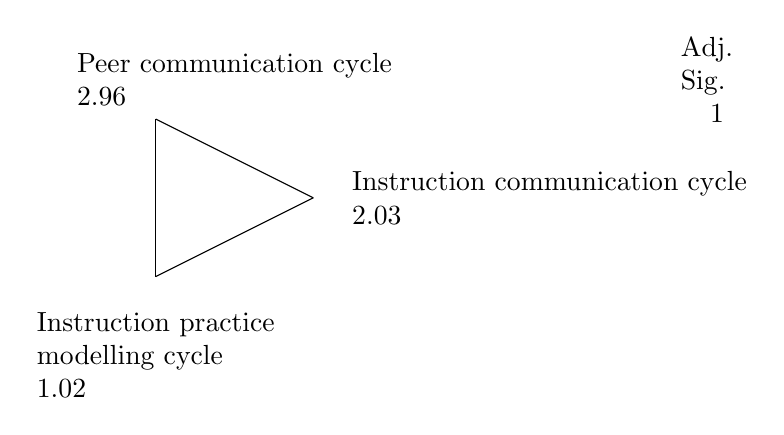
\begin{tikzpicture}[align=left]
\node(l) at (4,0) {Instruction communication cycle\\2.03};
\node(u) at (0,1.5) {Peer communication cycle\\2.96};
\node(d) at (-1,-2) {Instruction practice\\modelling cycle\\1.02};
\draw (1,0) -- (-1,1);
\draw (-1,1) -- (-1,-1);
\draw (-1,-1) -- (1,0);
\node at (6,1.5) {Adj.\\Sig.\\\sout{\hphantom{xx}}1};
\end{tikzpicture}}
\caption{\label{fig:porter:2}Pairwise comparison of ranked data for completed steps grouped by cycles (mean ranks). Each node shows the sample number of successes.}
\end{figure}

\begin{sloppypar}
Step engagement in the instructor communication cycle was significantly greater than step engagement in the instructor practice/modelling cycle, $\chi^2(2) = 1.006,\allowbreak p <0.0001$ (moderate effect size $ r= 0.50$). By contrast, step engagement in the instructor communication cycle was significantly lower than in the peer communication\slash modelling cycle, $\chi^2(2) = -0.930,\allowbreak p <0.0001$ (moderate effect size $r=-0.47$). The peer communication\slash modelling cycle also generated significantly more step engagement than the instructor practice\slash modelling cycle ($\chi^2(2) = -1.936,\allowbreak p <0.0001$, large effect size $r =-0.96$).
\end{sloppypar}

So, if step completion could reasonably be deemed an indicator of participant engagement, the data showed that cycles of steps linked to different aspects of the formal learning process influenced learners differently, with most engagement prompted by the peer communication/modelling cycle. This is interesting because participants were invited to make comments and be involved in all cycles. Recall that the peer modelling cycle principally involved two kinds of activities: videos where participants watched practising teachers explaining their own principled teaching practices and differentiated opportunities to evaluate others’ teaching or to discuss and experiment with their own pedagogic tasks. These kinds of steps were more successful at encouraging participants to engage fully with the content and to mark the step as complete.

\section{Discussion}\label{sec:porter:4}\largerpage[-2]

\begin{sloppypar}
For research question 1, the study set out to explore the extent to which research-informed professional development activities could change teacher beliefs, knowledge and practice. It is important to note here that the qualitative results presented relate to a partial analysis of the dataset. Nonetheless, we believe that the findings show emerging patterns.
\end{sloppypar}

\begin{sloppypar}
The evidence showed that changes in knowledge, understandings and beliefs were more prevalent in the data ($n=1755$ counts) than changes in practice (478 planned; 132 enacted). This is not unexpected as previous research has shown that changing teachers’ beliefs/knowledge is easier than realising adaptations in teaching practice, and that changes in the former generally precede the latter (as summarised in \citealt{MacaroEtAl2015}). Our findings supported a view that CPD has the potential to influence practice but, like \citet{CabarogluRoberts2000}, we sought a more nuanced view of change. However, while study sought to distinguish between change and modification, we explored whether changes were planned or enacted. We found that teachers were more likely to reflect on possibilities for change rather than report actual enactment of changes in practice. This, we believe, was largely driven by lockdown conditions enforced at the time of data collection but could indicate that other contextual (time constraints, curricular requirements) or individual factors (teacher confidence/expertise, motivation) might influence enactment of changes in practices.
\end{sloppypar}

The data also supported the \citet{MarsdenKasprowicz2017} view that teachers are interested in engaging with research and readily discussed and explored research: 23\% of comments coded showed discussion of MOOC research findings. Whilst the MOOC title mentioned research (``\ldots\,putting research into practice''), it was primarily advertised as: ``discover engaging, age-appropriate teaching methods and ideas to enhance your foreign languages teaching skills for children''. This, we believe, lends some weight to our interpretation that the research content, albeit explicitly linked to practice, was valued. However, it is important to note that the way in which research was presented might have facilitated such explorations. Firstly, the teachers viewed videos hosted by researchers which distilled findings into three or four distinct messages, framed as pedagogic principles. These steps showed the highest counts of changes in beliefs. Teachers were also able to access a weekly research reading using accessible language as well as ``teacher-friendly'' research summaries, hosted off-platform. In other words, considerable efforts were made to a) translate research findings into workable pedagogic suggestions and b) to distil research findings into clear and accessible formats. We suggest that the MOOC format offers an opportunity for ``international, systematic and sustainable'' practitioner engagement with research findings (\citealt[613]{MarsdenKasprowicz2017})

In terms of themes which emerged from the quantitative and qualitative data, participants’ views often reflected those noted in the literature, especially regarding lay wisdom and a lack of subject-specific pedagogic knowledge (\citealt{Barrios2014,GartonEtAl2011}). For example, comments relating to changes in beliefs/knowledge about developmental issues perhaps show that ToYLLs tended not to consider these in FL classrooms (\citealt{Hild2017,Rea-DickinsGardner2000}). Comment analysis also showed subject-specific knowledge deficits followed by awareness raising and improved understanding around: motivation and progression (\citealt{CourtneyEtAl2017}), how grammar is learned (\citealt{GrahamEtAl2017,KocamanCansiz2012,Roothoft2017}), multimodality (\citealt{MitchellMyles2019,MylesMitchell2012,Porter2020}) and FL literacy (\citealt{Porter2020}). The aforementioned studies have shown that these factors are likely to affect FL outcomes and are therefore important in primary FL pedagogy. It is important to note, however, when looking at frequency counts for patterns in the qualitative data, that the MOOC audience was diminishing each week. Therefore, engagement numbers need to be viewed as a proportion of active learners rather than as an indicator of overall engagement.

For research question 2, we set out to explore whether Laurillard’s framework for learning environment promoted the most learner engagement, evidenced by step completion metrics. Both the descriptive and inferential statistical analyses showed a particular tendency for step completion of the peer communication and modelling cycles to be greater than the instructor practice and instructor modelling cycles respectively. Learner comments also acknowledged the perceived usefulness of collaboration and co-construction with peers.

All the cycle data do demonstrate, however, the relative accessibility and potential for engagement of each cycle and its related steps. They also show that whilst attrition is a real issue for online CPD activities, those participants who joined each week were engaged and committed, completing most of the available steps and contributing rich and expansive comments. In other words, online CPD can be linked to the kinds of cycles of interaction proposed by Laurillard and suggest that the Conversation Framework could be a useful tool to examine the optimal conditions for participant engagement in online learning (\citealt{Laurillard2012}).

\section{Conclusion and implications for practice}

This study has shown that a short CPD course has the potential to influence teacher beliefs, knowledge and practice, albeit that this relies on reported instances of planned or enacted change. It suggests that scaffolded access to research, that is research produced in a teacher-friendly format with pedagogic models (in the form of principles and teacher stories) can be a useful tool to encourage change. It also found differences between planned and enacted change. This requires further empirical investigation to determine, for example, whether any, contextual or individual factors might support or impede enacted practice.

In terms of optimal learning design, our data suggested that accessible communication of new knowledge and generation of questions to explore concepts is likely to be helpful in underpinning professional development. However, further analyses, exploring participant interaction across a wider range of communication cycles, will enable us to better understand the contribution of the peer communication and modelling cycle to the teacher learning process.

On a broader level, our online CPD MOOC attracted a large and diverse global audience. We believe this supports the view that primary languages professionals are eager to bridge any gaps between their own beliefs and research findings. The contribution of Florence Myles to helping such professionals developing their understanding of early language learning cannot be overestimated, and we are proud to have worked with her on this MOOC initiative.

% % % % % \appendixsection{Teacher-friendly research findings summary access at \url{https://ripl.uk/research/}}\label{app:porter:a}
% % % % % %\begin{figure}
% % % % % \noindent
% % % % % \includegraphics[width=\textwidth]{figures/a8PorterGraham-img003.png}
% % % % % %\end{figure}


\appendixsection{Deductive coding framework for platform comments data}\label{app:porter:b}

\largerpage[3]
{\small\begin{longtable}{p{.5\textwidth} p{.5\textwidth}}
\lsptoprule {Parent Nodes} & {Child Nodes}\\ \midrule\endfirsthead
\midrule {Parent Nodes} & {Child Nodes}\\ \midrule\endhead
\endfoot\lspbottomrule\endlastfoot
Changes in teacher understanding: New or adapted understandings, beliefs, knowledge about:

{ }- change = new understandings\slash beliefs\slash knowledge

{ }- change = refined\slash adapted understandings/beliefs/knowledge

{ }- change = realisation\slash affirmation of existing tacit understandings\slash beliefs\slash knowledge & Developmental change during middle childhood

The importance of progression for motivation

Learning of grammar

Learning vocabulary

Multimodality

Planning for progression

Learning to read in the FL

Learning to write in the FL

Independent language use

Learning vocabulary

Multimodality\\
\midrule
Changes in teaching practice (planned)\slash expression of a desire to change, potential for change in teaching:

{ }- change = contrasting prior practices with future ones

{ }- change = additions to existing pedagogic repertoires

{ }- change = adaptations to existing pedagogic repertoires & To support motivation and\slash or engagement

To support language use

To support grammar teaching

To support use of multimodality

To support FL reading

To support FL writing

To support independent language use\\
\midrule
Changes in teaching practice (enacted): & To support language use

To support grammar teaching

To support use of multimodality

To support FL reading

To support FL writing

To support independent language use

To support independent language use\\
\midrule

MOOC as an opportunity for teacher learning: & Reported opportunities to share and collaborate

Actual sharing of practices between teachers

Newly designed activities through Padlet wall\\
\midrule
Explicit reflections on MOOC research content: & Articulation of research findings

Discussion of research findings

Request for clarification\slash explanation of research findings\\
\midrule
Explicit reflections on pupil learning: & Actual observations of changes in learning\slash outcomes

Expected changes in learning\slash outcomes\\
\end{longtable}}

\printbibliography[heading=subbibliography,notkeyword=this]
\end{document}
